\section{ Proprietà vibrazionali dei solidi}
Nella sezione precedente ci si è concentrati sulla dinamica degli elettroni, visti come pacchetti d'onda che si muovono in un potenziale periodico. L'attenzione ora verrà spostata alle proprietà vibrazionali del reticolo. Il sistema cristallino viene sempre considerato con la solita approssimazione adiabatica. Elettroni e nuclei hanno scale di tempo di evoluzioni molto diverse quindi possiamo sempre separare lo studio delle due componenti, appunto moto degli elettroni e moto dei nuclei. L'Hamiltoniana del sistema da studiare è
\newl{-\frac{\hbar^2}{2}\left(\sum_i\frac{\nabla^2_{R_i}}{M_i}\right)\psi(R) + U_{\text{ad.}}(R) \psi(R) - E\psi(R) = 0.}
Dove con $i, j$ si identifica l'indice di particella, mentre con le lettere greche $\alpha, \beta$ si indentifica l'indice di direzione.
Supponiamo che $\vet R_0$ sia il punto di equilibrio di sistema, in questo caso posso sviluppare il potenziale adiabiatico in un intorno di $\vet R_0$ 
\newl{U_{\text{ad.}} =U_0 +  \sum_{i,\alpha,j,\beta} \left(\frac{\partial^2 U_{\text{ad.}}}{\partial u_{i,\alpha} \partial u_{j,\beta}}\right)_{R_0} u_{i,\alpha} u_{j,\beta} = U_0 + \Phi_{i,\alpha, j, \beta} u_{i,\alpha} u_{ j,\beta}  }
La $\vet \Phi$ è chiamata \textit{Matrice delle costanti di Forza} e rappresenta l'approssimazione parabolica del potenziale adiabatico lungo le varie direzioni, quindi le forze di richiamo, in approssimazione quadrata, lungo i vari assi. Per scrivere l'equazione del moto dei nuclei si passa dalla lagrangiana del sistema in cui i vari nuclei sono legati da una forza di richiamo, lungo le varie direzioni, indicata dalla matrice delle costanti di forza $\vet \Phi$. Se il numero di particelle è $N$ avrò $3N$ equazioni 
\newl{\mathcal{L}= \frac{1}{2}M_i(\dersf{u} _{i,\alpha})^2 - \frac{1}{2}  \Phi_{i,\alpha, j, \beta} u_{i,\alpha} u_{ j,\beta} }
per comodità di notazione sostituisco $q_{i,\alpha} = u_{i,\alpha}$ in questo modo posso scrivere le equazioni di Lagrange nella solita forma
\newl{\frac{d}{dt}\frac{\partial \mathcal{L}}{\partial \dersf{q} } - \frac{\partial \mathcal{L}}{\partial q}=0 }
derivando si ottengono le equazioni del moto
\newl{M_i \derrsf{u} _{i,\alpha}  + \Phi_{i,\alpha, j,\beta}u_{j,\beta} =0 .}
Nella prima parte, la ripetizione dell'indice $i$ nella matrice delle masse e nella parte di velocità non è da intendersi come somma covariante, in realtà $i$ è un indice libero che non si somma. Risolvo l'equazione differenziale nello spazio $\vet k$, passo quindi alla trasformata di Fourier 
\newl{k^2 {\vet M} u(k)  - {\vet \Phi} u(k) = 0.}
Definisco per semplicità $w = \sqrt{{\vet M}} u$, ottenendo
\newl{k^2 w - \left(\sqrt{{\vet M}}\right)^{-1} {\vet \Phi} \left(\sqrt{{\vet M}}\right) w =0 .}
La matrice ${\vet D} = \left(\sqrt{{\vet M}}\right)^{-1} {\vet \Phi} \left(\sqrt{{\vet M}}\right)$ è comunemente conosciuta col nome \textit{Matrice Dinamica}. Non è necessariamente diagonale quindi si trova un  operatore che sia in grado di diagonalizzarla. Si supponga che esista un operatore identificato dalla matrice $\vet S$ che goda delle seguenti proprietà
\newl{{\vet S}^\dagger {\vet S} = {\vet 1}, \text{e renda diagonale: }  {\vet S}^\dagger {\vet D} {\vet S} = 
	\left(\begin{array}{c c c}
		w_1^2&  &  \\
		 & \ddots &  \\
		 &  & w_N^2 \end{array}\right)
.}
Le coordinate degli autovettori di ${\vet D}$ sono
\newl{q={\vet S}^\dagger w \implicaa q = {\vet S}^\dagger {\vet M} ^{\frac{1}{2}} u \implicaa u = {\vet M}^{-\frac{1}{2}} {\vet S} q.}
Riscrivo la lagrangiana nella nuova base diagnonale
\newl{\mathcal{L} = \frac{1}{2} \dersf{w} ^\dagger \dersf{w} -\frac{1}{2} w^\dagger {\vet D} w = \frac{1}{2} \dersf{q} {\vet S^\dagger} {\vet S}\dersf{q} -\frac{1}{2} q {\vet S}^\dagger {\vet D}  {\vet S} q  ,}
essendo tutto diagonale posso scrivere la Lagrangiana in funzione di un singono indice
\newl{\sum_\gamma \mathcal{L}_\gamma = \frac{1}{2} \sum_\gamma \left[ \left(\dersf{q} _\gamma\right)^2 -k^2_\gamma q_\gamma\right].}
Effettuando il cambio di variabili $Q_\gamma = \sqrt{w_\gamma} q_\gamma$ ottengo
\newl{\mathcal{L} = \frac{1}{2}\sum_i \left[\frac{\dersf{Q} _i^2}{w_i}-w_iQ_i^2\right],}
che è praticamente la lagrangiana di un oscillatore armonico, infatti tramaite trasformata di Legendre arrivo quasi alla tipica Hamiltonina di un oscillatore armonico
\newl{H = \sum_i w_i \left(\frac{\op{P_i} ^2 + \op{Q_i} ^2}{2}\right)}
che, per come è stato impostato il problema,  è un risultato abbastanza aspettato. Usando gli operatori di salita e discesa\footnote{che sono definiti come: $\op{a} _i^\dagger =\frac{1}{\sqrt{2\hbar}} \left(\op{Q} _i - i\op{P} _i\right)$ e $\op{a} _i = \frac{1}{\sqrt{2\hbar}} \left(\op{Q} _i + i \op{P} _i\right)  $. }  arrivo esattamente all'Hamiltoniana di un oscillatore
\newl{H=\sum_i\hbar w_i \left(\op{a} _i^\dagger \op{a} _i +\frac{1}{2}\right).}
Quanto scritto vale per un sistema di $N$ atomi senza tener conto della periodicità del reticolo. Introducendo il fatto che il sistema è periodico con periodicità quella del reticolo, per la matrice delle costanti di forza vale la seguente scrittura
\newl{\phi_{i,n\alpha, j,n'\beta} = \phi_{i,(n'+n")\alpha, j,(n'+n")\beta} .}
Data la periodicità del sistema posso scrivere gli stati come stati di Bloch costituiti quindi da una parte periodica, con periodicità del reticolo, e da una parte di onda piana. Nello spazio di Fourier lo stato di block è
\newl{
	&&\tildato{W} _{i,n\alpha} = \sqrt{M_i} u_{i,n\alpha}\nonumber\\
	&&u_{i,n\alpha} = \frac{\tildato{W} _{i,n\alpha}}{\sqrt{M_i}} =  \frac{W_{i,n\alpha}}{\sqrt{M_i}} e^{ikR}
}
Sostituendo gli stati di Bloch nella Lagrangiana, tramite le equazioni di E-L arrivo ancora all'equazione del moto nello spazio $k$
\newl{
	&&k^2{\vet M} u -{\vet \Phi}u =0\nonumber\\
	&&k^2M_i\frac{W_{i,n\alpha}}{\sqrt{M_i}} e^{ikR_n} - \Phi_{i,n\alpha,j,n'\beta} \frac{W_{i,n\alpha}}{\sqrt{M_i}} e^{ikR_n}=0 
}
che usando la periodicità può essere riarrangiata in una forma più evidente
\newl{ \left(k^2W_{i,\alpha}({\vet k})  - \Phi_{i,\alpha,j,(n'-n)\beta} \frac{W_{j,(n'-n)\beta}({\vet k})}{\sqrt{M_j M_i}}\right) e^{ikR_n}=0  }
\subsection{Reticolo monodimensionale a due atomi}
Un esempio applicativo di quanto detto fin'ora è rappresentato dal reticolo monodimensionale con due specie atomiche.

\begin{center}
	\fbox{
		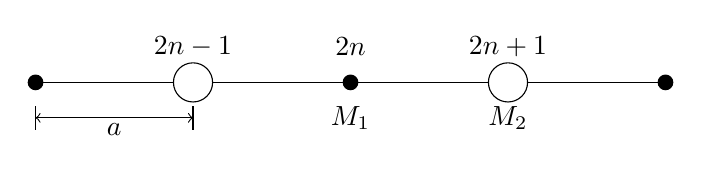
\begin{tikzpicture}[scale=1,auto=center]
			\draw (0,0) -- (1.75,0);
			\node[fill,thick,circle, inner sep=0pt, minimum size=0.2cm] at (0,0)  {};
			\node[draw, circle, inner sep=5pt, minimum size=0.1cm] at (2,0) {};
			\draw (2.25,0) -- (4,0);
			\node[fill,thick,circle, inner sep=0pt, minimum size=0.2cm] at (4,0)  {};
			\draw (4,0) -- (5.75,0);
			\node[draw, circle, inner sep=5pt, minimum size=0.1cm] at (6,0) {};
			\draw (6.25,0) -- (8,0);
			\node[fill,thick,circle, inner sep=0pt, minimum size=0.2cm] at (8,0)  {};


			\node[] at (2,0.45) {$2n-1$};
			\node[] at (4,0.45) {$2n$};
			\node[] at (6,0.45) {$2n+1$};
			\node[] at (4,-0.45) {$M_1$};
			\node[] at (6,-0.45) {$M_2$};

 			\draw (0,-0.3) -- (0,-0.6);
			\draw (2,-0.3) -- (2,-0.6);
			\draw[<->] (0,-0.45) -- (2,-0.45);
			\node[] at (1,-0.6) {$a$};


		\end{tikzpicture}
	}
\end{center}
I due atomi sono rappresentati dalle due diverse masse $M_1$ e $M_2$. La cella reticolare è di dimensione $2a$. Il fatto che siano presenti due tipi diversi di atomi questo permette di scrivere due equazioni del moto 
\newl{
	&&M_1 \frac{d^2u_{2n+1}}{dt^2} = -\alpha(2u_{2_n+1}-u_{2_n}-u_{2_n+2} )\\
	&&M_2 \frac{d^2u_{2n+2}}{dt^2} = -\alpha(2u_{2_n+2}-u_{2_n+1}-u_{2_n+3})
}
Dove $\alpha$ è la costante di accoppiamento interatomica, $n$ è un indice intero e scorre su tutti gli atomi di tipo $M_1$ quando è dispari e $M_2$ quando è pari. Le equazioni scritte sopra sono palesemente accoppiate. Abbiamo un totale di $2N$ equazioni differenziali accoppiate, da risolvere simultaneamente. Per risolvere questo tipo di equazioni si prende sempre in cosiderazione il sistema in studio e si formula un'Ansazt. Quella più attendibile è 
\newl{\left[\begin{array}{c}
		u_{2n+1} \\
		u_{2n}
\end{array}\right] = 
\left[\begin{array}{c}
	A_1e^{iqX_{2n+1}} \\
	A_2e^{iqX_{2n+2}}
\end{array}\right] e^{-i\omega t} .
}
In questo modo tutti gli atomi di massa $M_1$ hanno tutti ampiezza $A_1$ e lo stesso vale per gli atomi di massa $M_2$ che hanno ampiezza $A_2$. Sostituendo la soluzione del sistema di equazioni differenziali accoppiate scritto inizialmente, passando attraverso alcune drastiche semplificazioni si arriva alla semplice scrittura
\newl{\left(\begin{array}{cc}
		2\alpha - M_1\omega^2 & -2\alpha \cos(qa) \\
		-2\cos(qa) & 2\alpha -M_2\omega^2
	\end{array}\right) 
	\left(\begin{array}{c}
			A_1\\
			A_2
	\end{array}\right) = 0,
}
che è l'equivalente di due equazioni differenziali simulatanee nelle variabili $A_1$ e $A_2$. Le equazioni sono omogenee e hanno soluzione non banale solo se il determinante si annulla. La condizione diventa quindi
\newl{\text{det} \left|\begin{array}{cc}
	2\alpha - M_1\omega^2 & -2\alpha \cos(qa) \\
	-2\cos(qa) & 2\alpha -M_2\omega^2
	\end{array}\right| = 0.
}
A questa condizione corrisponde un'equazione nella variabile $\omega^2$ le cui soluzioni sono
\newl{\omega^2 =\alpha\left(\frac{1}{M_1} + \frac{1}{M_2}\right)\pm\alpha\sqrt{\left(\frac{1}{M_1} + \frac{1}{M_2} \right)^2 - \frac{4\sin^2(qa)}{M_1M_2}} .}
Come è possibile notare in Fig.~$\ref{PH:AC}$, in corrispondenza dei due diversi segni si distinguono due \textit{branches}, ottici e acustici.
\begin{figure}
	\centering
	\fbox{
		\begin{tikzpicture}[scale=1,auto=center]
			\draw[->] (0,0) -- (0,5);
			\draw[->] (-2.5,0) -- (2.5,0);
			\node[] at (0,5.3) {$\omega$};
			\node[] at (0,-0.25) {$0$};
			\node[] at (2,-0.25) {$\pi/2a$};
			\node[] at (-2,-0.25) {$-\pi/2a$};
			\draw[dashed] (2,0) -- (2,5);
			\draw[dashed] (-2,0) -- (-2,5);
			\draw[domain=-2:2] plot (\x,{3*sqrt((sin(\x*45))^2) });
			\draw[domain=-2:2] plot (\x,{3*sqrt((sin((\x+4.5)*20))^2)+1});
			
		\end{tikzpicture}
	}
	\caption{Fononi: bande acustiche e bande ottiche}
	\label{PH:AC}
\end{figure}
I rami acustici partono da $(0,0)$ e sono funzione crescente di $q$. Intorno a zero il comportamento è in prima approssimazione lineare, il che torna con le relazioni di dispersione lineare del suono nei mezzi, ben conosciuti in fisica calssica, la curva poi satura sui bordi della zona di Brillouin. Il ramo ottico invece, per $q=0$ vale 
\newl{\omega = \left[2\alpha\left(\frac{1}{M_1}+\frac{1}{M_2}\right)\right]^{1/2}} 
e descresce molto lentamente nell'avvicinarsi al bordo della zona di Brillouin. La frequenza di questo braccio non varia in modo apprezzabile lungo tutto il range di valori di $q$, infatti solitamente si considera costante. Il range di frequenze, tra la parte alta del ramo acustico e la parte bassa del ramo ottico, rappresenta una zona di frequenze non consentite. In questo range il cristallo non può trasmettere nessun tipo di onda. Il risultato che si ha è quello che ogni onda di frequenza proibita, che interagisce col cristallo, viene fortemente attenuata.
